\documentclass{exam}

\usepackage{amsmath,amssymb,amsfonts,amsthm,dsfont}
\usepackage{lib/extra}
\usepackage{graphicx}
\usepackage{tikz}
\usepackage{enumitem}
\usepackage{bbm}
\usepackage{pgfplots}
\usepackage{fontenc}
\usepackage{float}

\pgfplotsset{compat=1.18}

\title{Complex Numbers and the Complex Plane}
\author{Brandyn Tucknott}
\date{Last Updated: 23 September 2025}

\begin{document}
\maketitle

\section{Basic Properties}
A complex number is of form $z = x + iy$ where $x,y$ are real numbers and $i$ is imaginary
satifying $i^2 = -1$. We call $x$ the \textbf{real part} and $y$ the \textbf{imaginary part} 
of $z$. We write this as 
$$x = \re{z} \qquad \text{ and } \qquad y = \im{z}.$$

We also take note that real numbers are complex numbers with zero imaginary parts, and we call a 
complex number with zero real parts \textbf{purely imaginary}. We can visualize the complex plane
by identifying any complex number $z = x + iy$ with the point $(x, y)$ in the Euclidean plane. We
call the $x$-axis the \textbf{real axis} and the $y$-axis the \textbf{imaginary axis} (see Figure 1).

\begin{figure}[H]
    \centering
    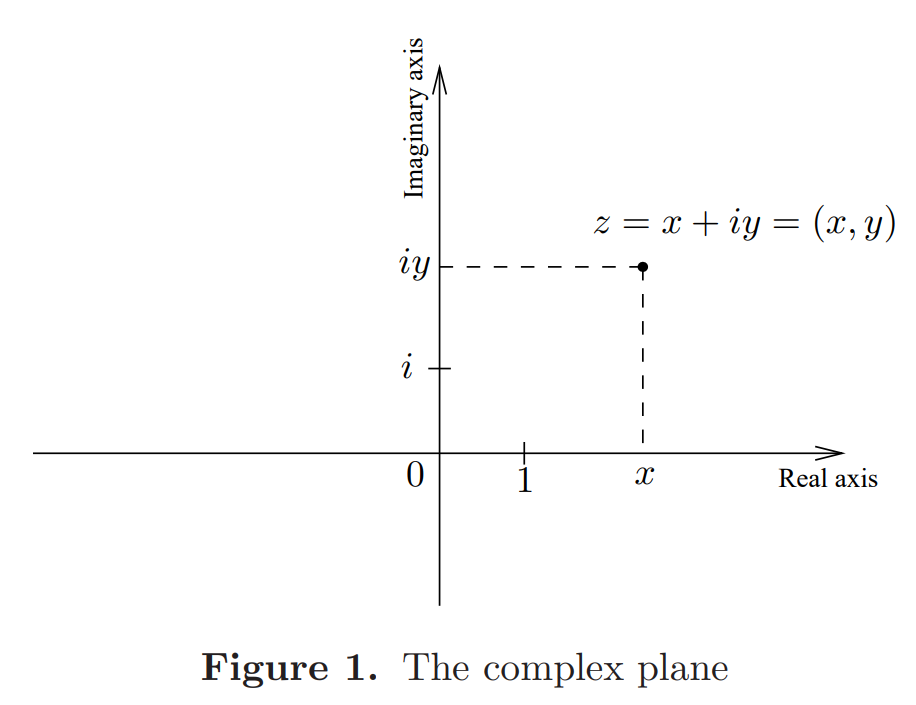
\includegraphics[width=0.5\textwidth]{figures/complex_analysis/figure_1.png}
    % \caption{The complex plane}
\end{figure}

The rules for adding and multiplying complex numbers can all be obtained by treating all numbers as
real numbers, noting that $i^2 = -1$. Below we show both rules and their derivations.
\begin{align*}
    z_1 + z_2 &= (x_1 + iy_1) + (x_2 + iy_2) \\
    &= x_1 + x_2 + iy_1 + iy_2 \\
    &= (x_1 + x_2) + i(y_1 + y_2)
\end{align*}

\begin{align*}
    z_1 z_2 &= (x_1 + iy_1)(x_2 + iy_2) \\
    &= x_1x_2 + x_1iy_2 + iy_1x_2 + i^2y_1y_2 \\
    &= (x_1x_2 - y_1y_2) + i(x_1y_2 + x_2y_1)
\end{align*}

\newpage

Using the two definitions above, we can verify that commutativity, associativity, and distributivity
hold for complex numbers.

\begin{align*}
    \text{Commutativity: }z_1 + z_2 &= (x_1 + x_2) + i(y_1 + y_2) \\
    &= (x_2 + x_1) + i(y_2 + y_1) \\
    &= z_2 + z_1
\end{align*}

\begin{align*}
    \text{Associativity: }(z_1 + z_2) + z_3 &= ((x_1 + x_2) + i(y_1 + y_2)) + (x_3 + iy_3) \\
    &= x_1 + x_2 + x_3 + iy_1 + iy_2 + iy_3 \\
    &= x_1 + iy_1 + (x_2 + x_3) + i(y_2 + y_3) \\
    &= z_1 + (z_2 + z_3)
\end{align*}

\begin{align*}
    \text{Distributivity: }z_1(z_2 + z_3) &= (x_1 + iy_1)((x_2 + x_3) + i(y_2 + y_3)) \\
    &= (x_1 + iy_1)(x_2 + x_3) + (x_1 + iy_1)i(y_2 + y_3) \\
    &= x_1x_2 + x_1x_3 + iy_1x_2 + iy_1x_3 + x_1iy_2 + x_1iy_3 + i^2y_1y_2 + i^2y_1y_3 \\
    &= (x_1x_2 - y_1y_2) + i(y_1x_2 + y_2x_1) + (x_1x_3 - y_1y_3) + i(y_1x_3 + y_3x_1) \\
    &= z_1z_2 + z_1z_3
\end{align*}

An astute reader may have noticed that addition and multiplication of complex numbers corresponds
with vector addition and dilated rotation. This fact will become more apparent when we introduce
the polar form of a complex number, but for now note that multiplication by $i$ corresponds
to a rotation by an angle of $\frac{\pi}{2}$.

The notion of length or \textbf{absolute value} is still the same, and thinking of complex numbers as vectors
for this purpose makes it easy to define the aboslute value (distance from the origin) of a
complex number:
$$|z| = \sqrt{x^2 + y^2}.$$

Here, we list some useful inequalities that hold for complex numbers. Let $\C$ denote the set of
all complex numbers. Then for all $z, w \in \C$, we have the following:
\begin{itemize}
    \item $|z + w| \leq |z| + |w|$ (Triangle Inequality)
    \item $|\re{z}| \leq |z|$ and $|\im{z}| \leq |z|$
    \item $||z| - |w|| \leq |z - w|$ (Reverse Triangle Inequality)
\end{itemize}


We define the \textbf{complex conjugate} of $z = x + iy$ to be the point reflected across the real
axis in the complex plane.
$$\overline{z} = x - iy.$$

A complex is real if and only if $z = \overline{z}$, and purely imaginary if and only if
$z = -\overline{z}$. 

By directly using the definitions of complex numbers and their conjugates, we can verify that
$$\re{z} = \frac{z + \overline{z}}{2}\qquad \text{ and } \qquad \im{z} = \frac{z - \overline{z}}{2i}$$
and also that
$$|z|^2 = z\overline{z} \longrightarrow \frac{1}{z} = \frac{\overline{z}}{|z|^2} \text{ whenever } z \neq 0$$

\newpage

We now introduce the \textbf{polar form} of a complex number. Any non-zero complex number can be written as
$$z = re^{i\theta}$$
where $r > 0$ and $\theta \in \R$. Here, $\theta$ is often called the \textbf{argument} of $z$, is
defined uniquely up to a multiple of $2\pi$, and is denoted by $\arg{z}$.

Another important definition,
$$e^{i\theta} = \cos{\theta} + i\sin{\theta}$$
and since $\abs{e^{i\theta}} = 1$, we see that $r = |z|$ with $\theta$ as the angle (with positive
counter clockwise orientation) between the real axis and the line segment from the origin to $z$.

\begin{figure}[H]
    \centering
    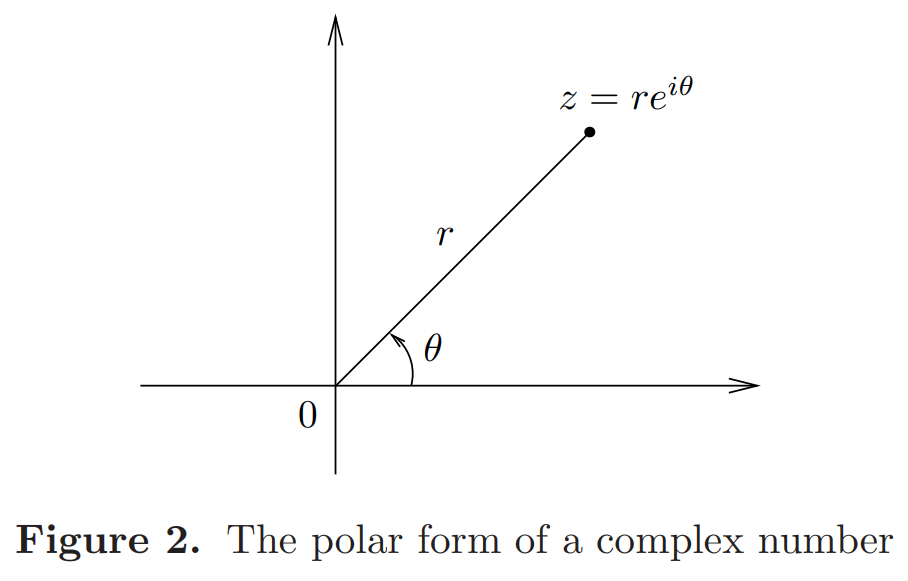
\includegraphics[width=0.5\textwidth]{figures/complex_analysis/figure_2.png}
\end{figure}

Finally, note that if $z = re^{i\theta}$ and $w = se^{i\phi}$, then
$$zw = rse^{i(\theta + \phi)},$$
which allows us to plainly see why multiplication of complex numbers corresponds to
dilated rotation in $\R^2$.

\section{Convergence}
left off on page 24 of pdf

\end{document}